\documentclass[draft, english]{volcanica-template}
\nonstopmode
% \doublespacing
\newcommand{\ArticleType}{Research article}			
% Please choose between Research article, Report, Review, or Methods. 
% Details about different article types are available at: 
% https://www.jvolcanica.org/ojs/index.php/volcanica/about/submissions

% To properly render supplement table of all model parameters
\usepackage{pdflscape}   % landscape pages
\usepackage{longtable}   % multi-page tables
\usepackage{makecell}    % \makecell[lt]{...}
\usepackage{colortbl}

%------------------------------------------------------------
%  Article details go here 
%------------------------------------------------------------	
\newcommand{\Title}{Supplementary information for: Thermodynamic modeling tools for the interpretation of melt inclusions and volcanic gases} 	% Manuscript title goes here.
\newcommand{\shortTitle}{Thermodynamic modeling of melt inclusions and volcanic gases} 		        % Short title for header goes here, less than 60 characters.
\newcommand{\Author}{Iacovino et al.\xspace}    	% First author goes here.

%------------------------------------------------------------
%  Author details go here 
%------------------------------------------------------------	
\author[{{\affiliation{1}}}] 				% affiliation number
{\orcidaffil{0000.0002.2461.7748}~			% orcid number
Kayla Iacovino	 				            % first author
\Email{kiacovino@seti.org}} 		        % corresponding author email

\author[{{\affiliation{2},\affiliation{3}}}] 				
{\orcidaffil{0000.0002.3445.281X}~			
Ery Hughes} 					        	

\author[{{\affiliation{4}}}] 				
{\orcidaffil{0000.0002.1070.8323}~			
Penny Wieser}

\author[{{\affiliation{5}}}] 				
{\orcidaffil{0000.0002.9263.622X}~			
Alain Burgisser}

\author[{{\affiliation{6}}}] 				
{\orcidaffil{0000.0003.2880.6711}~			
Philippa Liggins}

\author[{{\affiliation{7}}}] 				
{\orcidaffil{0000.0003.0365.2752}~			
Shuo Ding}

\author[{{\affiliation{8}}}] 				
{\orcidaffil{0000.0002.9768.2815}~			
Chenguang Sun}

\author[{{\affiliation{3}}}] 				
{Geoff Kilgour}

%------------------------------------------------------------
%  Affiliations 		
%------------------------------------------------------------	
\affil[{{\affiliation{1}}}]{
Carl Sagan Center for Research, SETI Institute, Mountain View, CA, 94043, US.
}

\affil[{{\affiliation{2}}}]{
Department of Earth Sciences, University College London, London, WC1E 6BT, UK.
}

\affil[{{\affiliation{3}}}]{
Earth Sciences New Zealand, Te Awa Kairangi ki Tai Lower Hutt, 3351, Aotearoa New Zealand.}

\affil[{{\affiliation{4}}}]{
Department of Earth and Planetary Science, University of California Berkeley, Berkeley, CA, US.
}

\affil[{{\affiliation{5}}}]{
Univ. Grenoble Alpes, Univ. Savoie Mont Blanc, CNRS, IRD, Univ. Gustave Eiffel, ISTerre, Grenoble, 38000, France.
}

\affil[{{\affiliation{6}}}]{
University of Oxford, Oxford OX1 2JD, UK.
}

\affil[{{\affiliation{7}}}]{
University of Florida, Gainesville, FL, 32611, US.
}

\affil[{{\affiliation{8}}}]{
University of Texas, Austin, TX, 78712, US.
}

%------------------------------------------------------------
%  BIBLIOGRAPHY FILE 		
%------------------------------------------------------------	  
\addbibresource{references.bib}		  		% add the name of the bibliography file here

%------------------------------------------------------------
%  Start of Document 		
%------------------------------------------------------------	  
\begin{document}

\maketitle

\section{List of Supplementary Materials}
All of these materials are available through the journal's repository and in the GitHub repo: \url{https://github.com/kaylai/volcanic-gas-modeling-tool-comparison}.
\begin{enumerate}
    \item This PDF
    \item All modeling results from all tools generated in this work: in folder ``\url{Model\_Outputs}''
    \item All modeling tool settings used to generate results: in folder ``\url{Model\_Outputs/resolved\_inputs}''
    \item Notebooks for creating every figure in this manuscript: in folder ``\url{Figure\_Notebooks}''
    \item Full datasets used to choose starting compositions for our four basaltic systems: ``\url{Melt\_Inclusions/melt\_inclusion\_datasets.xlsx}''
    \item Jupyter notebook for describing how starting compositions were chosen from the full datasets: ``\url{Melt\_Inclusions/Choosing\_MI\_Kilauea.ipynb}''
    
\end{enumerate}

\section{Abbreviations}

All models are given by name and full citation in the first appearance in the text and thereafter referred to by a model name or abbreviation only: ``Allison'' \parencite{Allison2019}, ``Eguchi'' \parencite{Eguchi2018}, ``Frost'' \parencite{Frost1991}, ``Gaillard'' \parencite{Gaillard2003}, ``Iacono-Marziano'' or ``IM'' \parencite{IaconoMarziano2012}, ``Kress and Carmichael'' or ``KC'' \parencite{Kress1991}, ``Liu'' \parencite{Liu2005}, ``Moore'' \parencite{Moore1998}, ``Muth'' \parencite{Muth2021}, ``Nash'' \parencite{Nash2019}, ``Shishkina'' \parencite{Shishkina2014}, and ``VolatileCalc'' or ``VC'' \parencite[referring to both the original model equations and the Excel VisualBasic app:][]{dixon1995, Newman2002}.

\section{Model Options}
All model options chosen for the calculations in this manuscript are listed in Table \ref{table:table_comparison-table}. Equilibrium constants are for the following reactions:

$K_{H_2O}$: H$_2$O = H$_2$ + 0.5O$_2$

$K_{CO_2}$: CO + 0.5O$_2$ = CO$_2$

$K_{H_2S-1}$: 0.5S$_2$ + H$_2$O = H$_2$S + 0.5O$_2$

$K_{H_2S-2}$: H$_2$S + 1.5O$_2$ = SO$_2$ + H$_2$O

$K_{SO_2}$: 0.5S$_2$ + O$_2$ = SO$_2$

$K_{CH_4}$: CO$_2$ + 2H$_2$O = CH$_4$ + 2O$_2$

$K_{OCS}$: 3CO + SO$_2$ = 2CO$_2$ + OCS

\noindent Modeling tool settings used to generate our results are included in the Supplement in the folder ``\url{Model\_Outputs/resolved\_inputs}''. Note that for Sulfur\_X, the user can define a value for the B constant term to tweak the relationship between Fe and S redox (e.g., to be consistent with XANES data for the system as performed here for Kīlauea). Because of a paucity of experimental data for C-O-H-S-bearing systems at $P$ < $\sim$250 bars, instability in the computed combined K$_D$ can trend to infinity in special or unusual cases \parencite{Ding2023}. To mitigate this, Sulfur\_X allows the user to specify an arbitrary increase in the combined K$_D$ value at each pressure for the lowest pressure steps. In our model runs, we iteratively adjusted this behavior as well as other computational settings that control solver convergence until obtaining a Sulfur\_X run with no or minimal low-pressure instability. 

\begin{landscape}
\scriptsize
\renewcommand{\arraystretch}{1.15}

% --- one place to control geometry -------------------------
\newlength{\firstcol}\setlength{\firstcol}{1.6cm}
\newlength{\toolcol}\setlength{\toolcol}{3.6cm}
% span width = all 6 column widths + 5 interior gaps (10\tabcolsep)
\newlength{\spanwidth}
\setlength{\spanwidth}{\dimexpr\firstcol+5\toolcol+10\tabcolsep\relax}

% center the longtable on the page
\setlength{\LTleft}{\fill}
\setlength{\LTright}{\fill}

% shaded full-width section header, defined once
\newcommand{\sectionrow}[1]{%
  \multicolumn{6}{@{}p{\dimexpr\spanwidth+2\tabcolsep\relax}@{}}%
  {\cellcolor[HTML]{D9D9D9}\textit{\textbf{#1}}}}

\begin{longtable}{p{\firstcol}p{\toolcol}p{\toolcol}p{\toolcol}p{\toolcol}p{\toolcol}}

% ---------- caption + first-page header --------------------
\caption{Model parameterizations used by each tool. See notes
and reference key below the table.}
\label{table:table_comparison-table}\\
\toprule
Parameter & VolFe & Sulfur\_X & D-Compress & MAGEC & EVo \\
\midrule
\endfirsthead

% ---------- header repeated on continuation pages ----------
\multicolumn{6}{@{}l}{\footnotesize\itshape Table
\ref{table:table_comparison-table}, continued.}\\
\toprule
Parameter & VolFe & Sulfur\_X & D-Compress & MAGEC & EVo \\
\midrule
\endhead

% ---------- footer on all but the last page ----------------
\midrule
\multicolumn{6}{r@{}}{\footnotesize\itshape continued on next page}\\
\endfoot

% ---------- footer on the last page -------------------------
\bottomrule
\endlastfoot

% ============================================================
\sectionrow{SOLUBILITY}\\
\addlinespace[2pt]
H$_2$O &
  H24 FigS2 * &
  IM12 Eq11$^1$ * &
  IM12 Eq11$^1$ * &
  IM12 Eq11$^2$ * &
  B15 Tab1-basalt * \\
CO$_2$ &
  $^{\xi,\zeta,\theta}$D95 $^{\psi}$TH94 * &
  IM12 Eq7$^1$ * &
  IM12 Eq7$^1$ * &
  IM12 Eq7$^1$ * &
  B15 Tab1-basalt * \\
S$^{2-}$ &
  O21 Eq10.34$^3$ * &
  D23 Tab3-RxnI &
  N/A &
  N99 Eq3 * &
  O21 Eq10.34 * \\
S$^{6+}$ &
  OM22 Eq12a$^3$ * &
  D23 Tab3-RxnII &
  N/A &
  N/A &
  N/A \\
SO$_2$ &
  N/A &
  N/A &
  B15 Tab1-basalt * &
  N/A &
  N/A \\
H$_2$S &
  H24 FigS6-basalt * &
  N/A &
  B15 Tab1-basalt * &
  N/A &
  N/A \\
H$_2$ &
  H24 TabS4-basalt * &
  N/A &
  B15 Tab1-basalt * &
  G03 Sec5.4 &
  G03 Sec5.4 * \\
CH$_4$ &
  A13 Eq7a &
  N/A &
  0 * &
  A13 Eq7a &
  A13 Eq7a \\
CO &
  H24 TabS4 &
  N/A &
  0 * &
  A15 Eq10 &
  A15 Eq10 \\
O$_2$ &
  N/A &
  N/A &
  0 * &
  N/A &
  N/A \\
S$_2$ &
  N/A &
  N/A &
  0 * &
  N/A &
  N/A \\
\addlinespace[6pt]

% ============================================================
\sectionrow{MELT SPECIATION}\\
\addlinespace[2pt]
Fe$^{3+}$/$\Sigma$Fe &
  KC91 EqA5+A6 &
  KC91 Eq7 &
  KC91 Eq7$^4$ &
  SY24 Eq6-9+Tab2 * &
  KC91 Eq7 \\
S$^{6+}$/$\Sigma$S &
  N/A * &
  \makecell[lt]{$^{\xi,\psi}$MW21 $^{\zeta}$MW21$^{5}$\\$^{\theta}$OM22 Eq13 *} &
  N/A &
  SY24 Eq10 * &
  N19 Eq11 * \\
\addlinespace[6pt]

% ============================================================
\sectionrow{FUGACITY COEFFICIENT}\\
\addlinespace[2pt]
H$_2$O &
  HP91 Eq4+6+A1-3+Tab1 * &
  SS92 * &
  HP91 EqA2-3 &
  PR76 Eq15 &
  HP91 \\
CO$_2$ &
  SS92 * &
  N/A &
  SS92 &
  SS92 &
  HP91 \\
SO$_2$ &
  SS92$^6$ * &
  SS92 &
  SS92 &
  SS92 &
  SS92 \\
H$_2$S &
  SS92$^7$ * &
  SS92 &
  SS92 &
  SS92 &
  SS92 \\
O$_2$ &
  SS92 * &
  N/A &
  SS92 &
  SS92 &
  SS92 \\
H$_2$ &
  SW64 Eq4 * &
  N/A &
  SW64 Eq4 &
  SS92 &
  SW64 Eq4 \\
CO &
  SS92 * &
  N/A &
  SS92 &
  SS92 &
  SS92 \\
CH$_4$ &
  SS92 * &
  N/A &
  SS92 &
  SS92 &
  SS92 \\
S$_2$ &
  SS92 * &
  N/A &
  SS92 &
  SS92 &
  SS92 \\
OCS &
  SS92 * &
  N/A &
  N/A &
  SS92 &
  N/A \\
\addlinespace[6pt]

% ============================================================
\sectionrow{EQUILIBRIUM CONSTANTS}\\
\addlinespace[2pt]
$K_{\mathrm{H_2O}}$ &
  OK77 Tab1-d &
  N/A &
  OK77 Tab1-d &
  SL22$^8$ &
  EVo RTD$^9$ \\
$K_{\mathrm{CO_2}}$ &
  OK77 Tab1-c &
  N/A &
  OK77 Tab1-c &
  SL22$^8$ &
  EVo RTD$^9$ \\
$K_{\mathrm{H_2S}\text{-}1}$ &
  OK77 Tab1-h * &
  N/A &
  OK77 Tab1-h &
  SL22$^8$ &
  EVo RTD$^9$ \\
$K_{\mathrm{H_2S}\text{-}2}$ &
  N/A &
  D23 Eq4 &
  N/A &
  N/A &
  N/A \\
$K_{\mathrm{SO_2}}$ &
  OK77 Tab1-f * &
  N/A &
  OK77 Tab1-f &
  SL22$^8$ &
  EVo RTD$^9$ \\
$K_{\mathrm{CH_4}}$ &
  OK77 Tab1-e * &
  N/A &
  OK77 Tab1-e &
  SL22$^8$ &
  EVo RTD$^9$ \\
$K_{\mathrm{OCS}}$ &
  M19 Eq8 &
  N/A &
  N/A &
  SY24$^8$ &
  N/A \\
\addlinespace[6pt]

% ============================================================
\sectionrow{OXYGEN FUGACITY}\\
\addlinespace[2pt]
NNO &
  F91 Tab1 &
  N/A &
  F91 Tab1 &
  H08 Tab7$^{10}$ &
  F91 Tab1 \\
FMQ &
  F91 Tab1-FM$\beta$Q * &
  F91 Tab1-FM$\beta$Q &
  F91 Tab1-FM$\beta$Q$^{11}$ &
  H08 Tab7$^{12}$ &
  F91 Tab1-FM$\beta$Q \\
Redox input options &
  \makecell[lt]{Fe$^{3+}$/$\Sigma$Fe\\FeO + Fe$_2$O$_3$\\$\Delta$FMQ\\$\Delta$NNO\\log$_{10}f$O$_2$\\S$^{6+}$/$\Sigma$S} &
  $\Delta$FMQ &
  $\Delta$NNO &
  \makecell[lt]{log$_{10}f$O$_2$\\Fe$^{3+}$/$\Sigma$Fe\\S$^{6+}$/$\Sigma$S\\$\Delta$IW\\$\Delta$FMQ\\$\Delta$NNO} &
  \makecell[lt]{Fe$^{3+}$/$\Sigma$Fe\\FeO + Fe$_2$O$_3$\\$\Delta$FMQ\\$\Delta$NNO\\$f$O$_2$ (bar)} \\
\end{longtable}

% ---------- notes, constrained to table width ----------------
\vspace{-0.5\baselineskip}
\begin{center}
\begin{minipage}{\spanwidth}
\footnotesize
Notes: Parameterisations used for all calculations, except where
specified for individual melt compositions: $^{\xi}$MORB,
$^{\zeta}$K\={\i}lauea, $^{\theta}$Fuego, and $^{\psi}$Fogo.
* Indicates other parameterizations are available within the tool.
$^1$Hydrous parameters; $^2$Hydrous web-app parameters;
$^3$Including H$_2$O dilution; $^4$At 1 bar; $^5$Using 6.5 as the
last constant value; $^6$As modified in Fig.~S1 of
\parencite{Hughes2023}; $^7$As modified in Fig.~S1 of
\parencite{hughes2024}; $^8$Based on NIST-JANAF tables
\parencite{janaf1996}; $^{9}$Based on JANAF tables
\parencite{janaf1998}; $^{10}$References of
\textcite{o1993thermodynamic,Frost1991}; $^{11}$For this study only
because not included in the original tool; $^{12}$References of
\textcite{Oneill1987}.

\smallskip
References: A13 \parencite{ardia2013}; A15
\parencite{armstrong2015speciation}; B15 \parencite{Burgisser2015};
D95 \parencite{dixon1995}; D23 \parencite{Ding2023}; EVo RTD
(\url{https://evo-outgas.readthedocs.io}); F91 \parencite{Frost1991};
G03 \parencite{Gaillard2003}; H08 \parencite{hirschmann2008-LEPR};
HP91 \parencite{holland1991}; H24 \parencite{hughes2024}; IM12
\parencite{IaconoMarziano2012}; KC91 \parencite{Kress1991}; M19
\parencite{moussallam2019}; MW21 \parencite{Muth2021}; N99
\parencite{nzotta1999}; N19 \parencite{Nash2019}; OK77
\parencite{ohmoto1977}; O21 \parencite{o2021thermodynamic}; OM22
\parencite{Oneill2022}; PR76 \parencite{peng1976}; SW64
\parencite{shaw1964}; SS92 \parencite{shi1992}; SL22
\parencite{Sun2022}; SY24 \parencite{Sun2024}; TH94
\parencite{thibault1994solubility}.
\end{minipage}
\end{center}
\end{landscape}\label{supp-table_comparison-table}

\section{How to cite models}
When using model results in a publication, the specific model used should be: 1. well justified (see main text section \ref{sec:futuremodel}; and 2. properly cited. The version of the code should be included; model options used within the tool should be clearly recorded and cited appropriately (including if implemented via another tool); and a notebook or script to recreate the calculations and all model results should be included as supplementary material. Here we provide an example suitable for a publication:

\begin{quote}
    Closed- and open-system degassing curves were modeled using VolFe v1.0 \parencite{Hughes2025volfe} using solubility functions from \textcite{hughes2024modeling, dixon1995,ONeill2021, Oneill2022, ardia2013}, fugacity coefficients from \textcite{shi1992,shaw1964,holland1991, Hughes2023, hughes2024}, homogeneous vapor equilibria constants from \textcite{ohmoto1977, moussallam2019}, Fe$^{3+}$/Fe$_T$ from \textcite{Kress1991}, FMQ and NNO buffers from \textcite{Frost1991}, and sulfide and anhydrite saturation from \textcite{ONeill2021, chowdhury2019effect,  wieser2023pysulfsat}. Specific equations used are detailed in Table \ref{tab:volfe-models}.  Parameterizations for model dependent variables were chosen where the calibration dataset most closely matched the composition of the MI of interest. Test calculations show that this selection of model dependent variables in VolFe is able to reproduce saturation pressures from the experiments of ``X'' to within 20\%, which are close in composition to our MI. A full list of model configuration options and notebooks for reproducing test calculations and modeling outputs presented here are in the Supplementary Material.
\end{quote}

\begin{table}[!thbp]
    \centering
    \caption{Parameterizations used for model dependent variables in degassing calculations using VolFe.}
    \label{tab:volfe-models}
    \begin{tabular}{ll}
        \toprule
        Variable &	Reference \\
        \midrule
        \multicolumn{2}{l}{Fugacity coefficients} \\
        \midrule
        O$_2$ &	\textcite{shi1992} \\
        CO &	\textcite{shi1992} \\
        H$_2$ &	\textcite{shaw1964} \\
        S$_2$ &	\textcite{shi1992} \\
        CO$_2$ &	\textcite{shi1992} \\
        H$_2$O &	Eq. (4, 6: T $>$ 673 K, A1-3) \& Table 1 in \textcite{holland1991} \\
        SO$_2$ &	\textcite{shi1992} as modified in Fig. S1 of \textcite{Hughes2023} \\
        CH$_4$ &	\textcite{shi1992} \\
        H$_2$S &	\textcite{shi1992} as modified in Fig. S1 of \textcite{hughes2024} \\
        OCS &	\textcite{shi1992} \\
        \midrule
        \multicolumn{2}{l}{Homogeneous vapor equilibrium constants} \\
        \midrule
        CO$_2$ &	Reaction (c) in Table 1 of \textcite{ohmoto1977} \\
        H$_2$O &	Reaction (d) in Table 1 of \textcite{ohmoto1977} \\
        SO$_2$ &	Reaction (f) in Table 1 of \textcite{ohmoto1977} \\
        CH$_4$ &	Reaction (e) in Table 1 of \textcite{ohmoto1977} \\
        H$_2$S &	Reaction (h) in Table 1 of \textcite{ohmoto1977} \\
        OCS &	Eq. (8) in \textcite{moussallam2019} \\
        \midrule
        \multicolumn{2}{l}{Solubility functions} \\
        \midrule
        H$_2$O$_T$ &	Fig. S2 in \textcite{hughes2024} \\
        CO$_{2,T}$ &	Bullet (5) in \textcite{dixon1995} \\
        H$_{2,mol}$ &	Basalt from Table S4 in \textcite{hughes2024} \\
        CO$_{mol}$ &	Table S4 in \textcite{hughes2024} \\
        CH$_{4,mol}$ &	Eq. (7a) from \textcite{ardia2013} \\
        *S$^{2-}$ &	Eq. (10.43) from \textcite{o2021thermodynamic} (including H$_2$O dilution) \\
        SO$_4^{2-}$ &	Eq. (12a) from \textcite{Oneill2022} (including H$_2$O dilution) \\
        H$_2$S$_{mol}$ &	Basalt from Fig. S6 in \textcite{hughes2024} \\
        \midrule
        \multicolumn{2}{l}{$f$O$_2$ related parameters} \\
        \midrule
        Fe$^{3+}$/Fe${_T}$ &	Eq. (A-5, 6) from \textcite{Kress1991} (no H$_2$O dilution) \\
        FMQ &	FM$\beta$Q in Table 1 of \textcite{Frost1991}\\
        NNO &	NiNiO in Table 1 of \textcite{Frost1991} \\
        \midrule
        \multicolumn{2}{l}{Other} \\
        \midrule
        S$^{2-}$CSS &	Eq. (10.34, 10.43, 10.45, 10.46) in \textcite{o2021thermodynamic} \\
        S$^{6+}$CAS &	Eq. (8) in \textcite{chowdhury2019effect} using PySulfSat v1.0.2 \parencite{wieser2023pysulfsat}  \\
        \bottomrule
\end{tabular}
\end{table}

\section{Vapor}
The vapor composition during degassing is quite different between different tools (Figure \ref{fig:vapcomp}). Here we expand on potential differences in the tools that may be contributing to these changes. 


\begin{figure}
    \centering
    
\includegraphics[width=1\linewidth]{figures/SuppFig_vapor_comp.png}
    \caption{Vapor composition against normalized $P$ for each system using the different tools.}
    \label{fig:vapcomp}
\end{figure}

\subsection{Homogeneous vapor equilibrium constants}

The equilibrium constants for homogeneous equilibria in the vapor ($K$, which are independent of $P$ and melt composition but depend on $T$) control the vapor composition at a given set of conditions and therefore differences in $K$ can cause variations between model outputs. These $K$ can be calculated from model results using the vapor composition ($x^v_i$ and $f_{O_2}$) at 1 bar when $\gamma_i$ = 1 (i.e., $f_i$ = $x^v_iP$ at 1 bar) according to:

\begin{equation}
    H_2(v) + 0.5O_2(v) = H_2O(v)
\end{equation}

\begin{equation}
    K_H = \frac{f_{H_2O}}{f_{H_2}f^{0.5}_{O_2}}=\frac{\gamma_{H_2O}x^v_{H_2O}P}{\gamma_{H_2}x^v_{H_2}Pf^{0.5}_{O_2}}
\end{equation}

\begin{equation}
    CO(v) + 0.5O_2(v) = CO_2(v)
\end{equation}

\begin{equation}
    K_C = \frac{f_{CO_2}}{f_{CO}f^{0.5}_{O_2}}=\frac{\gamma_{CO_2}x^v_{CO_2}P}{\gamma_{CO}x^v_{CO}Pf^{0.5}_{O_2}}
\end{equation}

\begin{equation}
    0.5S_2(v) + O_2(v) = SO_2(v)
\end{equation}

\begin{equation}
    K_S = \frac{f_{SO_2}}{f_{S_2}^{0.5}f_{O_2}}=\frac{\gamma_{SO_2}x^v_{SO_2}P}{\left ( \gamma_{S_2}x^v_{S_2}P \right )^{0.5} f_{O_2}}
\end{equation}

\begin{equation}
    CH_4(v) + 0.5O_2(v) = CO(v) + 2H_2(v)
\end{equation}

\begin{equation}
    K_{CH} = \frac{f_{CO}f^2_{H_2}}{f_{CH_4}f^{0.5}_{O_2}}=\frac{\gamma_{CO}x^v_{CO}P \left ( \gamma_{H_2}x^v_{H_2}P \right )^2}{\gamma_{CH_4}x^v_{CH_4}Pf^{0.5}_{O_2}}
\end{equation}

\begin{equation}
    SO_2(v) + H_2(v) = H_2S(v) + O_2(v)
\end{equation}

\begin{equation}
    K_{HS} = \frac{f_{H_2S}f_{O_2}}{f_{SO_2}f_{H_2}}=\frac{\gamma_{H_2S}x^v_{H_2S}Pf_{O_2}}{\gamma_{SO_2}x^v_{SO_2}P \gamma_{H_2O}x^v_{H_2}P}
\end{equation}

\begin{equation}
    OCS(v) = CO(v) + 0.5S_2(v)
\end{equation}

\begin{equation}
    K_{SC} = \frac{f_{CO}f^{0.5}_{S_2}}{f_{OCS}}=\frac{\gamma_{CO}x^v_{CO}P \left ( \gamma_{S_2}x^v_{S_2}P \right )^{0.5}}{\gamma_{OCS}x^v_{OCS}P}
\end{equation}

\noindent Although these specific reactions and $K$ may not have been used in the tools directly, these are six independent reactions that describe a vapor containing O$_2$, H$_2$, CO, S$_2$, H$_2$O, CO$_2$, SO$_2$, CH$_4$, H$_2$S, and OCS (i.e., no reaction can be made from a combination of the other reactions). Hence, this represents a minimum number of $K$ in the system. Equilibrium constants are only calculated if the tool outputs all required $x^v_i$ for a specific reaction (e.g., Sulfur\_X, D-Compress, and EVo do not include $x^v_{OCS}$ and therefore $K_{OCS}$ cannot be calculated) and if the system calculation reached $P \leq$ 1 bar (e.g., VolFe calculations for Fuego and MORB did not reach $P$ = 1 bar and therefore values are not calculated; Figure \ref{fig:eq_constants}). D-Compress and VolFe use \textcite{ohmoto1977}, whereas Evo and MAGEC use in-house versions based on NIST/JANAF databases. Implications of these variations are discussed in the main text.

\begin{figure}
    \centering
    
\includegraphics[width=1\linewidth]{figures/SuppFig_equilibrium_constants.png}
    \caption{Equilibrium constants for each tool and system (i.e., different temperatures). Calculated at $P$ = 1 bar as described in the text.}
    \label{fig:eq_constants}
\end{figure}

\subsection{Fugacity coefficients}

We can also use the $K_i$ equations to investigate the difference between $\gamma_i$ in the different tools, which only depend on $P$ and $T$ (i.e., not melt composition). Individual $\gamma_i$ cannot be calculated, but ratios of various combinations can be. If the ratios are similar, this suggests the tools are using similar $\gamma_i$ (although the $\gamma_i$ could be perfectly off-setting each other, but that would be unlikely). As for calculating $K_i$, the ratios of $\gamma_i$ are only calculated if all the necessary vapor species are calculated and the calculation reaches $\leq$ 1 bar as $K_i$ must also be calculated. 

\begin{figure}
    \centering
    
\includegraphics[width=1\linewidth]{figures/SuppFig_fugacity_coeffs.png}
    \caption{Ratios of fugacity coefficients ($\gamma_i$ calculated using equilibrium constant equations in the text)}
    \label{fig:fugacity_ceoffs}
\end{figure}

Most tools are using very similar values for $\gamma_{\rm{H_2}}$, $\gamma_{\rm{S_2}}$, $\gamma_{\rm{SO_2}}$, $\gamma_{\rm{H_2S}}$, and $\gamma_{\rm{OCS}}$, as can be seen by comparing $\gamma_{\rm{S_{2}}}^{0.5}/\gamma_{\rm{SO_{2}}}$, $[\gamma_{\rm {SO_2}}\gamma_{\rm {H_2}}]/\gamma_{\rm{H_2S}}$, and $\gamma_{\rm {OCS}}/[\gamma_{\rm {CO}}\gamma_{\rm {S_2}}^{0.5}]$ in Figure \ref{fig:fugacity_ceoffs}. This makes sense given all tools are using \textcite{shi1992} for $\gamma_ {\rm S_2}$, $\gamma_ {\rm SO_2}$, $\gamma_ {\rm H_2S}$, and $\gamma_ {\rm OCS}$. The differences for VolFe at low-$P$ for $\gamma_ {\rm SO_2}$ and $\gamma_ {\rm H_2S}$ are due to modifications described in \textcite{Hughes2023,hughes2024} and are therefore expected. Most tools use \textcite{shaw1964} for $\gamma_ {\rm H_2}$, except MAGEC that uses a modified version of \textcite{shi1992}, and therefore the similarity in $\gamma_ {\rm H_2}$ is good. Most tools use equations from \textcite{holland1991} (although not the same specific equations), except MAGEC that uses eq. (15) from \textcite{peng1976}, which are likely giving different values leading to the differences seen in $\gamma_ {\rm H_2}/\gamma_{\rm H_2O}$ (Figure \ref{fig:fugacity_ceoffs}). Values for $\gamma_{\rm CO_2}$, $\gamma_{\rm CO}$, and $\gamma_{\rm CH_4}$ seem similar between tools (e.g., $\gamma_{\rm {CH_4}}/[\gamma_ {\rm {CO}}(\gamma_{\rm{H_2}})^2]$ and  $\gamma_{\rm {CH_4}}/[\gamma_{\rm {CO_2}}(\gamma_{\rm{H_2}})^2]$) in Figure \ref{fig:fugacity_ceoffs}). All tools use \textcite{shi1992} for $\gamma_{\rm {CH_4}}$ and $\gamma_{\rm {CO}}$, and most also use this for $\gamma_{\rm {CO_2}}$, except EVo that uses \textcite{holland1991}. There appear to be some minor variations in  $\gamma_{\rm {CO}}/\gamma_{\rm {CO_2}}$, suggesting minor differences in $\gamma_{\rm {CO}}$ and/or $\gamma_{\rm {CO_2}}$.

 O$_2$ in the vapor is highly non-ideal, and the deviation from ideality, the fugacity coefficient ($\gamma$), is dependent upon $P$ and $T$. We can test whether models are treating the non-ideality of O$_2$ in the same way by calculating $\gamma_{\rm O_2}$ from the definition of fugacity as a function of $P$:
 \begin{equation}
    f {\rm O_2} = \gamma_{\rm O_2} \times x_{O_{2}}^{v} \times P.
 \end{equation}

\noindent $\gamma_{\rm O_2}$ is unity for an ideal gas, but deviates strongly for a real gas, particularly at high $P$ \parencite[e.g.,][]{shi1992}. Supplementary figure \ref{fig:gO2} shows nearly perfect overlap, with $\gamma_{\rm O_2}$ from unity at 1 bar up to $\sim$1.5 at 2,000 bars, meaning that this is not a factor in the divergence of computed redox variables and is expected given all tools use the model of \textcite{shi1992} for $\gamma_{\rm O_2}$. Hence, differences in $\gamma _{\rm O _2}$ are not driving differences between model outputs.

\begin{figure}
    \centering
    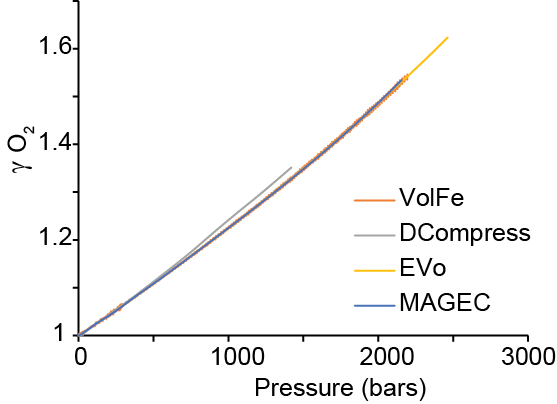
\includegraphics[width=1\linewidth]{figures/SuppFig_gO2.png}
    \caption{Non-ideal factor $\gamma$ for O$_2$ vs. pressure for four models.}
    \label{fig:gO2}
\end{figure}

\subsection{Molar mass balance in the vapor}
\label{sec:mol-balance-vapor}
One difficulty when using models from the literature is that some post-processing calculations cannot be carried out because they are at odds with either model assumptions or numerical limitations. The molar fraction of O$_2$ in the vapor, $x_{O_{2}}^v$, is a prime example of such limitations. Sulfur\_X does not include O$_2$ in the vapor calculation and therefore is not included in the following discussion. All other models assume that the sum of the molar fractions of all species in the vapor is equal to one, and thus one should be able to deduce the fraction of one species by calculating one minus the sum of all the others species. $x_{O_{2}}^v$ is notoriously small (typically $10^{-15}$--$10^{-11}$), whereas $x_{H_{2}O}^{v}$ is typically $10^{-1}$. This means that numerical limitations may be encountered because most models report (and calculate) in double precision ($\sim$15 significant digits). Figure \ref{fig:mO2} shows $x_{O_{2}}^v$ calculated by difference versus $x_{O_{2}}^v$ values output by the models. The bottom row shows the residual of the closure calculation $\Sigma$$x_i^v - 1$ (the sum of all vapor species minus 1) at each $P$ using Kīlauea as a representative example. 

D-Compress uses Turbo Delphi 2006 with TuboPower SysTools BCD allowing for floating point precision to 26 significant digits. All other models use Python or MATLAB's default double precision (IEEE 754 binary64) which is precise to 15–17 significant digits. This matters when very small values are converted between decimal representation (as we read it) and binary (as the computer reads it). Our plotted $x_{O_{2}}^v$ by difference and residual values were likewise computed in binary64 from each model's CSV output, meaning that residuals below this floor cannot be resolved regardless of how the values were computed internally. In other words, any trailing digits are meaningless noise from rounding error. 

D-Compress closure shows symmetric noise at the $\sim$$10^{-17}$ level scattered around zero, reflecting only float64 rounding caused by our by-difference calculation and indicating higher precision within the model itself. The closure plot in EVo reveals systematically negative residuals $\sim$$10^{-16}$–$10^{-17}$, indicating a normalization step within the solver capping sums to one. At reducing conditions below log$f$O$_2$ of -15 ($\sim\Delta$IW-3), $x_{O_{2}}^v$ cannot be recovered by-difference. Data by difference from MAGEC oscillate between negative and positive and, for that reason, we plot the absolute value in the 1:1 figure for MAGEC. The MAGEC output files used in this comparison were exported to 5 significant figures, resulting in the closure error of $\sim$$10^{-5}$–$10^{-6}$. Each species is rounded independently at output time, so per-$P$ step sign distributions are random and centered on zero (output-format rounding, not algorithmic bias). This does not indicate anything wrong with MAGEC's internal solver, but this output precision means that $f$O$_2$ cannot be reliably recovered by difference from the exported MAGEC outputs used here. Most VolFe outputs reflect the same expected double-precision behavior as EVo but show closure failure in certain cases, specifically for high-CO$_2$, low-H$_2$O points at the mid-$P$. This is likely the result of its iterative Newton-Raphson solver converging on a near-solution and exiting before normalization of gas species to one can be enforced. Adjusting the solver tolerance dependent upon composition could improve the recoverability of $x_{O_{2}}^v$ in certain cases.

High precision is not typically required to answer geologic questions, but the impact can be significant due to repeated computation within the code itself before a result gets returned to a user. Likewise, if precision is truncated when the code writes results to disk, any calculation those values are fed back into will never be better than the number of truncated digits, and this would almost certainly go undetected, since floating point error thereafter will mask the previous truncation. It is also worth flagging floating point rounding behavior in Microsoft Excel. Although computations within Excel adhere to IEEE 754 binary64, when any value is \textit{displayed} in the user interface, it is truncated to 15 significant figures, replacing the final two with zeroes. Additionally, if a file with numbers exceeding 11 digits is \textit{saved} from Excel, it's ``General'' format defaults to scientific notation and may silently drop several significant figures from all values \parencite{griffiths2022}. This effect has been noted as particularly damaging for data analysis in the genome biology literature \parencite{ziemann2016}.

%% MOLAR MASS BALANCE FIGURES %%
\begin{figure}
    \centering
    
\includegraphics[width=1\linewidth]{figures/SuppFig_o2_mass_balance_combined.png}
    \caption{Molar fraction of O$_2$ in the vapor as reported by modeling tools vs. calculated by difference for all models that report it: D-Compress, EVo, MAGEC, and VolFe. Some by difference values computed for MAGEC were negative and so we plot the absolute values in order to plot on a logarithmic axis. The bottom row shows the residual of the closure calculation (the departure from zero of the sum of all vapor species minus 1) for Kīlauea runs.}
    \label{fig:mO2}
\end{figure}
%%%%%%%%%%%%%%%%%%%%%%%

%% solubilities %%
\begin{figure}
    \centering
    
\includegraphics[width=1\linewidth]{figures/SuppFig_solubilities.png}
    \caption{Volatile proportionality factors (eq. 15 with all tools for all basalts showing the change in H$_2$O, CO$_2$, reduced S (S$^{red}$), and oxidized S (S$^{ox}$) proportionality factors ($H'_{i}$) as a function of pressure during degassing.}
    \label{fig:all-sol}
\end{figure}

\EndMatter
\end{document}